\begin{frame}{Simulaciones}
  \framesubtitle{Sistema: dos peatones en curso de colisión}
  \begin{columns}[c]
    \begin{column}{0.64\textwidth}
      \centering
      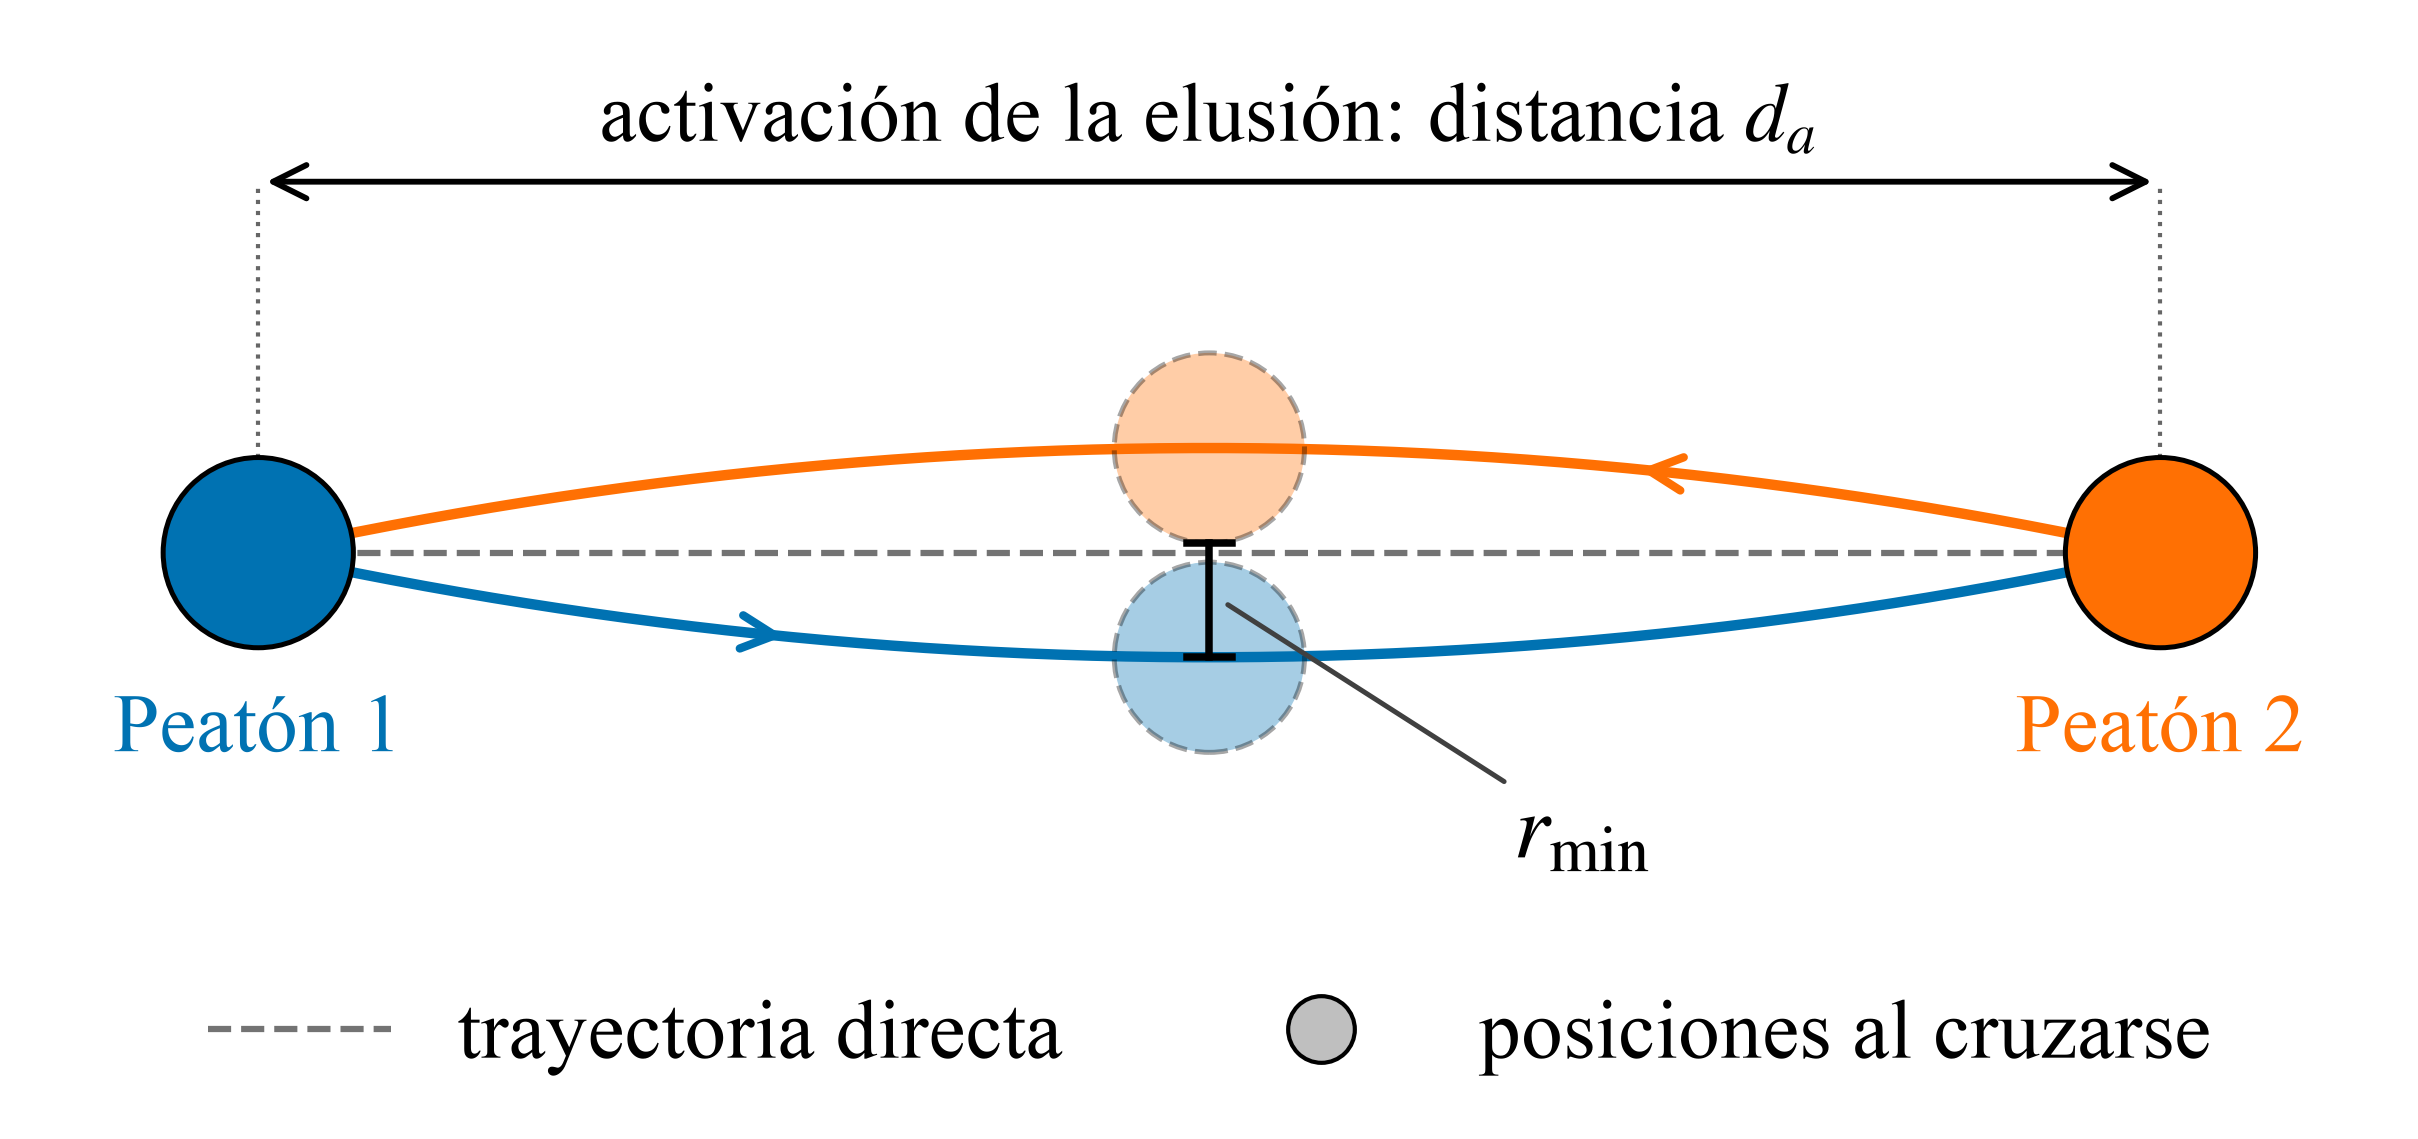
\includegraphics[width=\linewidth,height=0.72\textheight,keepaspectratio]{cuadro_inicial.png}
    \end{column}
    \begin{column}{0.33\textwidth}
      \begin{beamercolorbox}[wd=\linewidth,sep=8pt,rounded=true]{block body alerted}
        \small\textbf{Parámetros a calibrar}\par\vspace{6pt}
        $p_1 = d_{\mathrm{lat}}$: margen lateral de referencia\par\vspace{6pt}
        $p_2 = d_{\mathrm{act}}$: distancia de activación de la elusión
      \end{beamercolorbox}
    \end{column}
  \end{columns}
\end{frame}

\begin{frame}{Simulaciones}
  \framesubtitle{Eventos experimentales y parámetros fijos}
  \begin{columns}[c]
    \begin{column}{0.54\textwidth}
      \begin{beamercolorbox}[wd=\linewidth,sep=8pt,rounded=true]{block body}
        \small\textbf{Eventos experimentales}\par\vspace{4pt}
        \begin{itemize}\setlength{\itemsep}{6pt}
          \item $M = 18$ eventos, intervalo de muestreo $\Delta t_{exp} \approx 0.0666\uni{s}$
          \item Por evento: $\vv{r}_i(0)$, $\vv{v}_i(0)$, $v_{di}$ y $t_f$
          \item Target final: posición inicial del otro peatón
          \item $5$ eventos espejados: $y' = 2\,y_0 - y$
        \end{itemize}
      \end{beamercolorbox}
    \end{column}
    \begin{column}{0.38\textwidth}
      \begin{beamercolorbox}[wd=\linewidth,sep=8pt,rounded=true]{block body}
        \small\textbf{Parámetros fijos}\par\vspace{6pt}
        \renewcommand{\arraystretch}{1.25}
        \begin{tabular}{@{}l@{\qquad}l@{}}
          Radio $r_i$ & $0.25\uni{m}$ \\
          Masa $m_i$ & $80\uni{kg}$ \\
          $\tau_i$ & $0.5\uni{s}$ \\
          $k_n$ & $1.2\ten{5}\uni{N/m}$ \\
          $k_t$ & $2.4\ten{5}\uni{kg/(m\,s)}$ \\
        \end{tabular}\par\vspace{4pt}
        {\footnotesize Helbing et al. (2000)}
      \end{beamercolorbox}
    \end{column}
  \end{columns}
\end{frame}

\begin{frame}{Simulaciones}
  \framesubtitle{Observables}
  Error del peatón $i$ del evento $m$ \ ($N_m$ instantes $t_k = k\,\Delta t_{exp}$):
  \[
    E^{(1)}_i = \frac{1}{N_m}\sum_{k}\big|\vv{r}^{\,exp}_i(t_k) - \vv{r}^{\,sim}_i(t_k)\big|^2
    \qquad\quad
    E^{(2)}_i = \frac{1}{N_m}\sum_{k}\min_{j}\big|\vv{r}^{\,exp}_i(t_k) - \vv{r}^{\,sim}_i(t_j)\big|^2
  \]
  \vspace{2pt}
  Error del evento y error poblacional:
  \[
    E_m = \frac{E_1 + E_2}{2}
    \qquad\quad
    \langle E\rangle(d_{\mathrm{lat}},\,d_{\mathrm{act}}) = \frac{1}{M}\sum_{m=1}^{M} E_m(d_{\mathrm{lat}},\,d_{\mathrm{act}})
  \]
  \vspace{2pt}
  Barra de error: desvío estándar muestral entre eventos, \ $\langle E\rangle \pm \sigma_E$
  \[
    \sigma_E = \sqrt{\frac{1}{M-1}\sum_{m=1}^{M}\big(E_m - \langle E\rangle\big)^2}
  \]
\end{frame}

\begin{frame}{Simulaciones}
  \framesubtitle{Simulaciones realizadas}
  \textbf{Grilla de parámetros}
  \begin{itemize}\setlength{\itemsep}{3pt}
    \item $d_{\mathrm{lat}}$: $0.10$ a $0.50\uni{m}$, paso $0.05\uni{m}$ \ ($9$ valores)
    \item $d_{\mathrm{act}}$: $2.5$ a $7\uni{m}$, paso $0.5\uni{m}$ \ ($10$ valores)
    \item $90$ puntos de grilla $\times$ $18$ eventos $= 1620$ simulaciones
    \item Duración: $t_f$ de cada evento \ ($5.3$ a $8.9\uni{s}$)
  \end{itemize}
  \vspace{8pt}
  \textbf{Estudios} (por métrica)
  \vspace{3pt}

  \centering
  \begin{tabular}{ll}
    \hline
    Calibración poblacional & mínimo de $\langle E\rangle$ en la grilla, $18$ eventos \\
    Calibración individual  & mínimo de $E_m$ en la grilla, por evento \\
    Validación cruzada      & $20$ particiones al azar: $13$ de entrenamiento, $5$ de validación \\
    \hline
  \end{tabular}
\end{frame}
